Cuckoo filters provide a way of filtering elements with lower space overhead than counting filters while still allowing for deletion. While they are not as closely related to Bloom filters as counting filters are, and so we do not have the precise lower bound that \textit{any} attack against a Bloom filter also works against a cuckoo filter, it is true that since cuckoo filters are set-membership structures the specific bounds given in the Bloom filter section apply here. To establish acceptable upper bounds, we consider the case of a salted cuckoo filter with private representations. By `salted', we mean that both the hashing and the fingerprinting makes use of a salt chosen on a per-represntation basis. Using this definition, we can make use of the lemmas that allow us to talk about the structure in the single-represntation case with true random functions. A bound for the false positive rate in cuckoo filters is given by $\binom{n}{2k+1}\left(\frac{2}{2^f \cdot m}\right)^{2k}$ for a set of $n$ elements in a filter with $m$ buckets holding up to $k$ entries each, with fingerprint size $f$.

\begin{theorem}[Correctness Bound for Cuckoo Filters]\label{thm:cuckoo-salt-bound}
Fix integers $n, b, k, \lambda, r\geq 0$, where $m \geq \lambda$.
  For every $t, q_R, q_T, q_U, q_H \geq 0$ such that $q_T \geq r$, it holds that
  $$\Adv{\erreps}_{\struct,r}(t, q_R, q_T, q_U, q_H) \leq q_R \cdot
     \left[
      \frac{q_H}{2^\lambda} +
      {\dbinom{q_T+q_U}{r}} P(n,m,b,k+r)^r
    \right]$$
where $P(n,m,b,k)$ is the standard, non-adaptive false-positive probability on a cuckoo filter with those parameters.
\end{theorem}

\begin{figure}
  \boxThmBFSaltCorrect{0.48}
  {
    \underline{$\G_0(\advA)$}\\[2pt]
      $\col \getsr \advA^H$; $\setC \gets \emptyset$; $\err \gets 0$\\
      $\pub \getsr \Rep[\HASHO](\col)$\\
      $\bot \getsr \advA^{\HASHO,\QRYO,\UPO}$\\
      return $(\err \geq r)$
    \\[6pt]
    \oraclev{$\QRYO(x)$}\\[2pt]
      if $x \in \setC$ then return $\bot$\\
      $\setC \gets \setC \union \{x\}$\\
      $a \gets \Qry[\HASHO](\pub, \qry_x)$\\
      if $a \neq [x \in \col]$ then $\err \gets \err + 1$\\
      return~$a$
    \\[6pt]
    \oraclev{$\UPO(x,b)$}\\[2pt]
      $\setC \gets \emptyset$\\
      $a \gets \Qry[\HASHO](\pub, \qry_x)$\\
      if $x \in \setC$ and $a \neq [x \in \col]$ then\\
      \tab $\err \gets \err-1$\\
      if $b = 1$ then\\
      \tab $\col \gets \col \cup \{x\}$\\
      else\\
      \tab $\col \gets \col \setminus \{x\}$\\
      $\pub \gets \Up[\HASHO](\pub,\up_{x,b})$\\
      return~$\bot$
    \\[6pt]
    \oraclev{$\HASHO(x)$}\\
      $\hh \getsr [m]^2$; $\vv \gets \fff(\hh$)\\
      if $T[x]$ is defined then $\vv \gets T[x]$\\
      $T[x] \gets \vv$;
      return $\vv$
  }
  {
    \underline{$\G_1(\advA)$}\\[2pt]
    \oraclev{$\QRYO(x)$}\\[2pt]
      $\setC \gets \emptyset$\\
      $a \gets \Qry[\HASHO](\pub, \qry_x)$\\
      if $a \neq [x \in \col]$ then\\
      \tab $\err \gets \err+d(a,[x \in \col])$\\
      if $b = 1$ then\\
      \tab $\col \gets \col \cup \{x\}$\\
      else\\
      \tab $\col \gets \col \setminus \{x\}$\\
      $\pub \gets \Up[\HASHO](\pub,\up_{x,b})$\\
      return~$\bot$
    \\[6pt]
    \oraclev{$\UPO(x,b)$}\\[2pt]
      $\setC \gets \emptyset$\\
      $a \gets \Qry[\HASHO](\pub, \qry_x)$\\
      if $a \neq [x \in \col]$ then\\
      \tab $\err \gets \err+d(a,[x \in \col])$\\
      if $b = 1$ then\\
      \tab $\col \gets \col \cup \{x\}$\\
      else\\
      \tab $\col \gets \col \setminus \{x\}$\\
      $\pub \gets \Up[\HASHO](\pub,\up_{x,b})$\\
      return~$\bot$
  }
  {
  }
  {
  }
  \caption{Games 0--3 for proof of Theorem~\ref{thm:cuckoo-salt-bound}.}
  \label{fig:cuckoo-salt-bound}
\end{figure}

\begin{proof}
Again we can use lemma~\ref{lemma:errep} and lemma~\ref{lemma:salttorand} to reduce to the case of $\erreps1$ with true random functions in place of salted hash functions. We use this as the first game $\G_0$, so that $\Adv{\erreps}_{\struct_s,r}(\advA) \le q_R \cdot \left(\frac{q_H}{2^\lambda} + \Prob{\G_0(\advA) = 1}\right).$.

Because membership tests rely on objects having the same fingerprint, and a single bucket may contain multiple copies of the same fingerprint, deleting $n$ false positives can only produce up to $n$ false negatives, one per fingerprint removed. Unless the filter becomes full, it is therefore never helpful for an adversary to delete a false positive, since it cannot increase the number of errors. We may then assume, subject to the condition that the adversary never has to worry about the filter becoming full, that the adversary only makes insertion updates. Furthermore, we may assume the adversary never inserts elements which are already in the set, or elements which have already been queried and found to be false positives, since these also cannot increase the number of errors.

We want to show that alternating between sequences of queries and updates is no better than making updates first and queries afterwards. We have shown that the adversary only makes two types of updates: inserting unqueried elements which are not in the set and inserting known true negatives.

We move to a second game where each $\QRYO$ call also inserts that element. Additionally, the penalty for adding known false positives is removed. To avoid penalizing the adversary by producing an overly-full filter which rejects further insertions, we also increase the size of each bucket by $r$. Because we may assume without loss of generality that the adversary stops after finding $r$ errors, only $r$ false positives will be inserted and so these extra $r$ slots in each bucket are sufficient to ensure that if the buckets in the original game did not fill then the buckets in this game will not fill. Furthermore, we modify $\UPO$ to query for the element before inserting it. This cannot produce a worse result for the adversary, and so $\Prob{\G_0(A) = 1} \le \Prob{\G_1(A) = 1}$. Since $\QRYO$ and $\UPO$ calls are identical and each call is independent of all previous calls, the adversary's probability of success is exactly the probability of accumulating $r$ random errors from queries. Each query is a standard random query to a cuckoo filter, so by the binomial theorem we can get a bound of $\binom{q_T+q_U}{r}P(b,k+r)^r$. This gives the result:

$$\Adv{\erreps}_{\struct_s,r}(\advA) \le q_R \cdot \left(\frac{q_H}{2^\lambda} + \binom{q_U+q_T}{r}P(n,m,b,k+r)^r\right).$$\missingqed

\end{proof}

As with the other data structures, the graphs show how each of the parameters affects the adversarial advantage. The default parameters are $k = 4$, $m = 256$, $n = 100$, $f = 4$, $r = 10$, $q_R = 1$, and $q_H = q_T = q_U = 100$.

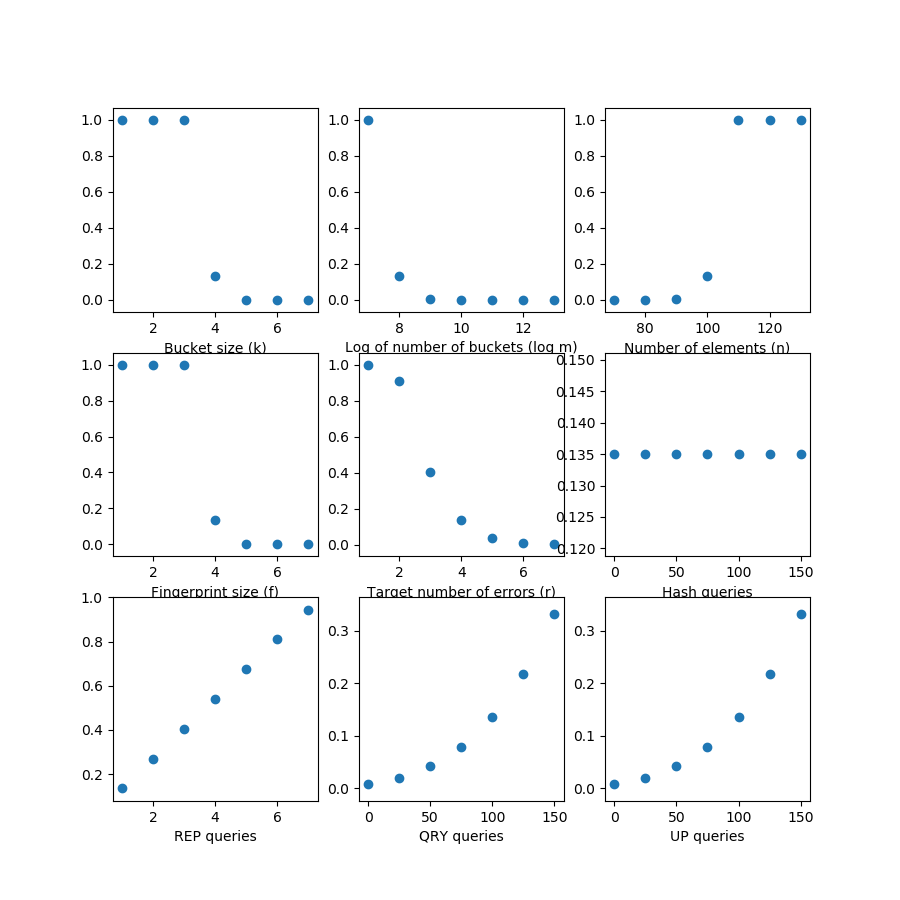
\includegraphics[scale=0.75]{CuF_Fig}